\chapter{Implementation}

Ensuing the chapter about the specification over WiFi, we will now address the implementation of the prototype. This chapter has been divided in 3 sections, each containing a number of subsections. We initiate with the plan of action which clearly states the trajectory this implementation will follow. Secondly we focus on the implementation of a Shim DIF prototype over WiFi. Finally we approach the subject of the Android implementation. 

\section{Plan of action}

%Section detailing the course that will be followed through this chapter. This shows a guide for the reader which allows the reader to understand the different steps taken in the implementation.

In this section we will give the reader a short introduction to the implementation topic. After this introduction we have the procedure of implementation. This subsection will detail the path followed for this entire implementation and will clearly show the milestones on the path. The section can be seen as a guide to understand the different steps taken in the implementation part. 

\subsection{Introduction}

%Quick introduction to reiterate the research question and how this implementation will try to help to answer it

The research question states: ``How to run RINA on Android over WiFi?''. Now that the background of this question has been clearly evaluated we can move towards the implementation. This chapter seeks to find a way towards a technical implementation of this research question. The chapter will not instantly address the question, but will start with some basic proof of concepts and already working implementations. After these have been carefully explained on how they were achieved, we move further towards the WiFi part of the research question and finally altering the operating system (OS) to Android. 
\npar
In the end we hope to have a working, technical implementation of the IRATI project code that can be constructed and applied to the given test devices\footnote{Test devices = 2x Samsung Galaxy S II smartphones}.

\subsection{Procedure of implementation}

%Define the exact procedure that will be followed of the implementation. Starting with setting up test bench with first 2 virtual devices that run the test provided by IRATI. Then try proof of concept over WiFi, if needed with two physical notebooks, if possible, install wifi device virtual and implement virtual again. After this is done, brief explanation on how to compile android kernel with glibc. Then the android kernel with glibc and the irati stack. Final steps involve the installation of this kernel on the target devices. 

In the final part of this section we will discuss in detail how the implementation will be addressed. For this, we reference to figure~\ref{fig:poi-flowchart}. This figure shows us clearly all the steps that will be talked about in this chapter. The steps with higher importance to this thesis will be specified and will be addressed in greater detail. 

\npar

\begin{figure}[H]
    \centering
    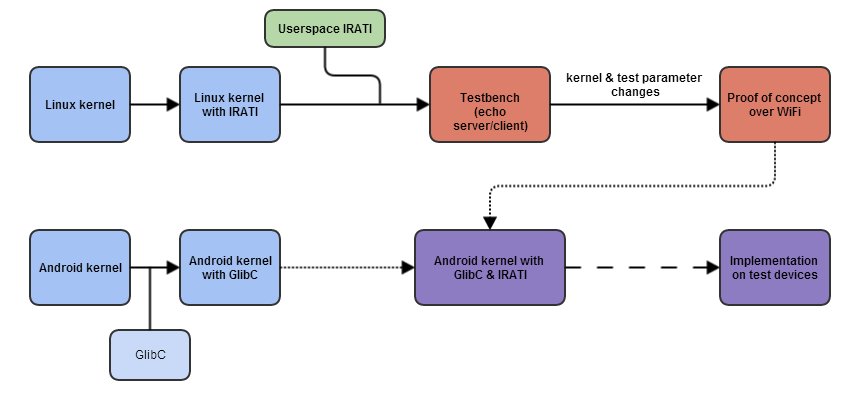
\includegraphics[width=1\textwidth]{figures/procedureofimplementation}
    \caption{Procedure of implementation - flow chart} 
    \label{fig:poi-flowchart}
\end{figure}

\npar

First we start with a proof of concept over WiFi. For this we use 2 linux machines who communicate through a simple echo program using RINA. This is an initial proof of concept that is needed to prove the capability of using RINA on top of WiFi. The point is here to prove that even though the WiFi frames are reformed to Ethernet frames by the drivers we can use these Ethernet frames for RINA. This is done by adding a VLAN interface (802.1Q) and using the Ethernet Shim DIF on top of this. This Ethernet Shim DIF and its functions are provided by the IRATI project. 
\\
The section initiates with an explanation on kernel compilation, where we briefly touch on how to build and install kernels. This a very basic step in the implementation that will see further use throughout the rest of the implementation chapter. Following this we prove the functionality of the Ethernet Shim DIF by setting up two virtual machines with RINA-enabled kernels that have the Ethernet Shim DIF. These are basic linux kernels with additions from the IRATI project. Finally we realize the proof of concept over WiFi. For this we use the linux kernels with both RINA and the IRATI additions enabled, plus the wireless parts added. 


\npar
After we have implemented a working RINA on pure linux machines, we initialize the process again on Android. We first note that also in Android the WiFi frames are transformed to Ethernet frames and only after this has been handled the user can use these frames. Specifically this means that once the kernel has been sufficiently modified for functionality on Android, that the wireless part is in essence the same as on pure linux computers. 
\\
Initially we explain how to build a basic android kernel and the differences to building a pure linux kernel. Secondly we explain how the IRATI-specific kernel parts are added to this base Android kernel. After this step we move towards adding the userspace implementation of the IRATI project. Because of previously mentioned limitation we require certain libraries so the addition of  glibc or a similar library will be required. Following this, we explain how the required userspace packages are added and how the userspace is configured. Once we are able to insert the modules and turn on the ipcmanager we can call this implementation a success. For the final part we explain the changes required to move from this basic Android kernel to a device specific kernel and run the echo experiment on the two test devices. 
\npar
We provide steps along this route on how we got to these parts, why we chose certain items over their respective alternatives and finally provide initial results to prove the functioning aspects of these implementations. 


\section{Proof of concept over WiFi}

In this section we will explain the implementation of the proof of concept of RINA over WiFi. This includes the compilation of a Linux kernel, the irati test bench setup and finally we show the proof of concept. 

\subsection{Compiling a kernel}

The first step of the implementation is building a base kernel. For this step we have several possibilities and guides available. While we will not go into details such as listing exact commands we intend to give a clear structure on how to build a basic kernel for a Linux Operating System. The reason we choose Linux is fairly straightforward:

\begin{itemize}
	\item Stable basic versions
	\item Under GNU General Public License, thus opensource code
	\item Big development community
	\item Crossplatform interoperabilities
	\item \ldots
\end{itemize}

We choose the most recent kernel version which can be found at \url{http://www.kernel.org}. After downloading and extracting this kernel we acquire all the needed packages to build this kernel. For a Debian based system, these include:

\begin{itemize}
	\item kernel-package
	\item libncurses5-dev
	\item fakeroot
	\item wget
	\item bzip2
	\item bc
\end{itemize}

These packages are Debian specific, but a quick online search should state which packages are required for the specific Linux system. After acquiring these packages one can follow a few simple steps, set up the configuration file and have the kernel built. Consequently you can install the kernel next to the current one and select which kernel you prefer on boot. This has several advantages which include always have a stable base kernel to fall back upon. It also allows the addition of new code to the kernel in several, testable stages. Further information on how to build kernels can be found in Appendix B~\ref{chap:app-b}.

\subsection{Test bench irati}
\label{ssec:test-bench-irati}

%Current irati implementation, what the differences are with a stock kernel and what exactly modules are. Finally show the code to run the test.

The current IRATI implementation consists of a Linux Kernel with RINA added in kernelspace and some additions to the Userspace which are closely linked to the Kernel. The modifications to the kernel are mostly additions to the \emph{net} section of the kernel. This is in essence the RINA implementation. Because this implementation is the Shim DIF over 802.1Q we also need to add the VLAN option in the configuration file. After adding these kernel files and selecting their options in the config file we can build the kernel in the same manner as in the previous subsection. Finally we are also required to add the wireless drivers for to this kernel. For this we first find out which WiFi device our hardware has by running a simple \emph{lpci} command. A quick Google search gives us the needed kernel drivers and these options are selected in the configuration file. 
\\
The files needed to for this kernel are provided in addendum on physical storage alongside this thesis. However for optimal results we recommend acquiring the most recent files directly from the source. For general kernel files this is \url{www.kernel.org} and for the irati project this is \url{www.irati.eu}. 
\npar
The userspace part requires some added specific packages before it can be built and installed. These packages are:

\begin{itemize}
	\item maven
	\item libnl-genl-3-dev
	\item libnl-3-dev
	\item libtool
	\item autoconf
	\item openjdk-6-jdk
	\item git
	\item swig ($>$2.0.8)
\end{itemize}

The packages are again Debian specific and the correct packages should be acquired for the relevant Linux system. Because this code is still very sensitive to changes we refer to the IRATI project again for the most recent requirements. After acquisition of the these packages we can run the commands to install this userspace section. 
\npar
Initial test for this are run on 2 32-bit Debian Wheezy virtual machines. After we install both the correct kernel and add the IRATI userspace implementations to that, we set up the network between the two virtual machines. For this we add a virtual Ethernet device to both virtual machines and put them both in the same virtual network. As an additional test we also supply them with IP addresses which allows us to test basic ping commands to be sure that the machines can reach each other. While it is not necessary for RINA, it adds an extra check to confirm the connection between the network devices of the virtual machines. 
\npar
Following the setup of the network devices we insert the Loadable Kernel Module (LKM), \emph{802.1q}. This can be done when the system is booting or when the user requires it. When this module is up we can create a new network between the devices with a virtual tag (number). This tag acts as the DIF name for the Shim DIF. Once the link has been set up between the two devices, we initiate the RINA aspects of the test. We insert \emph{shim-eth-vlan} and \emph{normal-ipcp}. If these modules are activated properly, which can be checked in the log file of the kernel, we can move to the next step. This step involves running the ipcmanager, which is located in the userspace folder. Once this us brought up successfully on both devices, we can start communication between these machines. For testing purposes we use a simple echo-server on one machine and an echo-client on the other. This lets us test the communication between the two machines. 

\subsection{Proof of concept over WiFi}

%Show how to add WiFi devices to a virtual machine and use those to test the irati stack over WiFi, if only bridging can work and no internal virtual wifi network can be set up (can this be done easily?) just run two linux notebooks with fresh kernel + irati.

Finally we implement the proof of concept over WiFi. For this we need to note that in Linux and Linux-like kernels, WiFi frames are reconstructed to Ethernet headers. This is done by the drivers, either accomplished in hardware (hardmac) or by software (softmac). Once these frames have been transformed they are presented to the kernel. The kernel has in essence no knowledge that these frames are WiFi frames. In our proof of concept this can be seen as an advantage because we can reuse the IRATI code and create a virtual interface (802.1Q) that is directly linked to the WiFi device. Normally the wireless device is called \emph{wlan0}, after the creation of the virtual device we simply add a virtual device: \emph{wlan0.number}, where the number is the VLAN tag. This VLAN tag is the Shim DIF name.
\npar
The setup for the proof of concept over WiFi is fairly similar to the one with the virtual machines. However for this we add the wireless device drivers in the kernel and use two physical devices. The reason we use physical devices is because virtual machines cannot have virtual wifi devices. The reason for this is that virtualization software packages such as VirtualBox, which was used for this thesis, cannot present WiFi frames to the virtual machine. 
\npar
After the setup of both kernels and the relevant userspace, we can run the test. This test is the same test we ran on the virtual devices and proves the communication between the two physical devices over WiFi. For this test we set up an ad-hoc network with static IP addresses (unrelated to RINA) which gave us certainty that the devices could reach each other. The proof of communication can be found on the physical media in the logfiles.

\section{Android implementation}

In this section we will address the implementation of RINA on Android. We initiate with a subsection about Android kernels, more specifically moving towards the device specific kernel. This includes the judgments that had to be made when selecting kernels, the issues that arose during these processes and finally the proof of implementation. After this subsection we move to the Android compilation with the irati kernel stack and which complications presented themselves during this process. Following this section we address the Android compilation with glibc, a requirement to run the userspace section of the IRATI codebase. We then move towards the final step of the Android implementation with both the kernel and userspace implementation. Here again we note the issues, choices and obstacles that present themselves when implementing this subsection. Finally we offer the alternative possibilities to the implementation, their advantages and their disadvantages. 
\npar
Note that we have set up an implementation process that might not be suitable at this time of implementation. This could be due to arising problems, which would force us to search for alternatives. This does not mean that implementation is impossible, but simply not possible within the current scope of the Master's Thesis. A similar note had to be made when it came to the Wireless stack, which had to be abandoned because implementing full hardware drivers for entire 802.11 was outside the scope of this Thesis. 

\subsection{Android kernel}

The first subsection is dedicated to the implementation of an Android kernel. While this process is very similar to the basic Linux kernel, some very specific additions are required to build these kernels. 
\\
Unlike the Linux kernel, is the Android kernel fairly device specific. Android kernels are provided by the producer of the smartphone and are iterated upon from that point on. In most cases this means that the kernel is almost never updated compared to the more recent Linux kernels. This can be instantly noted with our kernel. The version of this kernel is 3.0.101, at the time of writing (June 2014) the most recent Linux kernel is 3.16.x. The only update that was brought to this kernel during the entire Thesis was an upgrade from version 3.0.64 to 3.0.101. A fairly minor update in essence. These Android kernels are specifically tailored to each device. Most changes in these kernels comes from optimization processes by community developers who try to squeeze a bit more out of the kernel. Examples of this could be: updating specific files, changes hardware settings, adding modules to improve functionality, \ldots. Since Android devices are almost never modular, adding different device drivers quickly becomes useless these developers. And while the newest kernels could support the newest hardware, this is simply not needed for these ``older'' devices which rely on a basic, stable kernel. 
\npar
For our device, \emph{Samsung Galaxy SII - i9100}, we opted to go for the Cyanogenmod ROM with a modified Apolo\footnote{\url{http://forum.xda-developers.com/galaxy-s2/development-derivatives/kernel-t2291756}} kernel. The following reasoning was used: cyanogenmod was chosen because several reasons. These are:

\begin{itemize}
	\item Large development community
	\item Most recent version of Android supported (4.4.2) (stable)
	\item Decent guide to construct the ROM yourself
	\item Many kernels specifically designed for this ROM
\end{itemize}

The most recent build, with explanations on how to construct it yourself can be found here: \url{http://wiki.cyanogenmod.org/w/I9100\_Info}. The build we use in this thesis is Milestone 7 (M7), which is considered stable. With this ROM (Operating System) also comes a prepacked kernel. However for the purpose of this Master's Thesis we want to build our own kernel. The reason for this is fairly simple: we want control over the kernel so we can later add further code to it. In this environment this code is the IRATI code alongside the requirements to run the IRATI code, such as VLAN and the correct wireless network devices. 
\npar
The kernel we chose for this project is the Apolo Kernel, branch 7.0b, specifically tailored to Cyanogenmod (CM). The kernel can be found here: \url{http://forum.xda-developers.com/galaxy-s2/development-derivatives/kernel-t2291756}. The reasons for choosing this Apolo kernel are the following:

\begin{itemize}
	\item Stable base kernel with minor branching for user based optimization
	\item Updated codebase for the most recent CM build
	\item Large development community
	\item Good explanation on how to build the kernel yourself
\end{itemize}

This clearly shows the reasons why we chose this kernel. We have to note that other kernels that are built for Cyanogenmod Milestone 7 are fairly similar and could be considered almost equal to this kernel. Since we plan to add code to the kernel we first have to be able to build this basic kernel from scratch ourselves. This involves forking the repositories of both the initramfs and the kernel to our own github. These repositories can be found at: \url{https://github.com/mathieudevos/Kernel-smdk4412} and \url{https://github.com/mathieudevos/Initramfs_CM_4.4.x}. 
\npar
Before we can build these kernels we should briefly explain what initramfs is. Initramfs is the abbreviation for: ``initial ram file system''. This is the first file system that gets loaded into RAM on start-up. For basic Linux systems these are fairly straightforward. For Android they are very specific, up to the point where you need to exactly match your kernel and ROM with this initramfs. For this reason we select the initramfs based on Cyanogenmod for Android 4.4.x. When we take a closer look at the kernel in the github repository, we note a mk.sh file which automatically makes the correct zImage. This zImage is the image of our kernel that we need to flash over the current kernel. This image depends on the constructed kernel and on the initramfs. Some minor changes are required before we can run this shell script. These steps include, but are not limited to:

\begin{enumerate}
	\item Switch to the wip-md branch in the kernel repository. This is the work in progress branch which contains some minor changes.
	\item Change the name of the initramfs folder to match the forked repository. Thus changing it to ``initramfs''. 
	\item Further steps involving kernel building on Android (see Appendix~\ref{chap:app-b})
\end{enumerate}

The changes that are made to this kernel involve two patches. These patches affect the cypress keyboard device drivers, which is needed to utilize the hardware keys and the cl\_cfg80211 file. After these patches are applied, one can run the mk.sh file and acquire a new zImage that can be flashed as a kernel on the devices. When successful, you should see similar information in the ``About phone'' section of settings menu:
\npar
\begin{figure}[H]
    \centering
    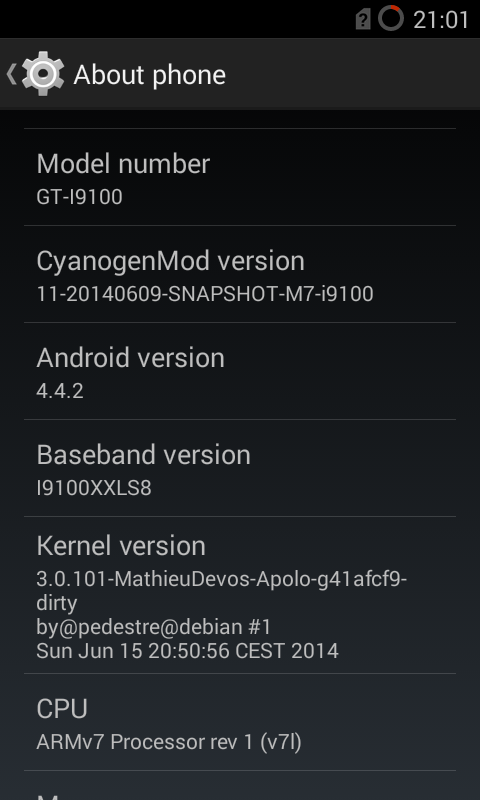
\includegraphics[width=0.5\textwidth]{figures/screenshot-kernel-i9100}
    \caption{Screenshot of ``About phone'' section of settings} 
    \label{fig:screenshot-kernel-i9100}
\end{figure}

\npar

Before we can move on to other subsections we have to note that this step is a very large step in the process and depending on the device, the support, the community, \ldots this can be a very lengthy process. We remark that this subsection, while now described simple, was quite a time-sink before we got to a working base kernel. This subsection is no longer as simple as just running the commands exactly as described on a website, so patches are needed, changes of files, and most of all: testing if the kernel will actually boot. If you find that the kernel gets stuck on boot, we note that Android does have any early boot warning system. However to access this system we need to set up a serial console with USB-to-UART converter. For this reason we strongly recommend to use matching code (kernel $\leftrightarrow$ ROM) which has been recently updated. 

\subsection{Android kernel with IRATI kernel code}

When we finally obtain the basic stable Android kernel with the code to build it, we can move towards adding the IRATI code to it. This subsection is only dedicated to the IRATI kernel code addition. Before we can implement the userspace, we first need a working kernel with all the correct kernel-specific code.
\npar
To add to this base kernel we use the git repository from IRATI over linux. Since Android is based on Linux we consider this to be a good starting point. The IRATI stack uses a base kernel and builds further on upon this. This means that when we create a patch that finds the differences between the base kernel and the IRATI kernel, we only have IRATI specific changes. This patch can then be applied to the base Android kernel in steps.
\npar
The patch will try to create new files when needed, change files or delete files which are no longer needed. However several issues arise here. In the current implementation of Linux, one can add system calls to the syscall table, called syscall\_32.tbl or syscall\_64.tbl depending on the architecture. These tables can be found in \emph{arch/x86/syscalls/}. However, this simply does not exist in our Android kernel. Not only does the file not exist, the map is simply non-existent. According to a guide\footnote{\url{http://www.techipost.com/2012/08/30/steps-of-adding-system-call-to-linux-kernel/}} we found on the Internet, we should be able to add these to unistd\_32.h. This is currently untested as we simply did not get this far yet because we have found issues with other files.
\npar
During the Make phase of the kernel we found ourselves stuck with the \emph{rmap.c} file. This calls for a hashtable function. This is where the first issue shows up. Hashtables are not implemented in Android, at least not in C. The solution to this was a fairly quick hack where we copied the hashtable.h file from a standard Linux kernel to the Android kernel. Now the function could be found, but we still had issues with one of the functions. The function: \emph{hlist\_for\_each\_entry\_safe} gives us the following error during compilation:
\\

\begin{lstlisting} 
net/rina/rds/rmap.c:87:68: error: macro "hlist_for_each_entry_safe" requires 5 arguments, but only 4 are given 
\end{lstlisting}

A quick glance at the code shows us that we are in fact passing 5 arguments to this function. Together with the previous issue of having difficulties of having to add system calls to the kernel, we are required to note that this might require an alternative approach. Since the user space implementation requires this kernelspace implementation to be functioning, the userspace subsection below has not been implemented in code as of yet. Due to the complexity of implementation that arose we are required to look for alternatives that will address both kernel- and userspace issues.

\subsection{Android compilation with glibc and IRATI userspace}

%First subsection about how to compile a base android kernel with glibc. Show steps taken to complete this process.

In this subsection we address the implementation of GlibC alongside Android. The reasons why we cannot stay with the same standard C library is fairly logic. Bionic, the C library for Android, does not provide full fledged support for \cpp, more on this can be read in the literature study~\ref{ssec:android-restrictions}. Simply said, if we want to install the userspace of IRATI, we will need access to a full C library. Several options are available here:

\begin{itemize}
	\item GNU C Library (glibc)
	\item dietlibc
	\item $\mu$clibc
	\item EGLIBC
\end{itemize}

We opted to for the most common library GlibC, because after further research we noted that this was the only one that had been implemented in Android. However it has never been done for the test devices, thus no previous experience could be relied upon. 
\\
After the implementation of the library we face another problem. Before the installation of the userspace can commence, we need some additional packages. The packages are freely available on Debian Wheezy systems. The packages are listed in the subsection, test bench irati (~\ref{ssec:test-bench-irati}). While these packages can be simply acquired from the source by running the standard ``apt-get install'' command (on Debian), this is unavailable in Android. The problem here is not that this command is OS-specific, it is that this command will also automatically check all dependencies for these packages. Furthermore is it possible that these packages do not support the ARM architecture, or are simply incompatible with the Android Operating System. 
\npar
Fixing this would require recompiling shell with GlibC so we would have a fully fledged shell with all commands. Next we would have to cross-compile every package and their dependencies separately. Then we would have to carefully install these packages on an alien system and hope that we would have the full functionality and commands available from these packages. This is clearly outside the scope of this Master's Thesis. Again, we need to look for an alternative. If this alternative is implementable within the timeframe of this Thesis is unknown.
\npar
A final remark about this userspace section of IRATI code. Currently the userspace section of IRATI provides RINA through the use of \cpp code. This can be seen in the figure~\ref{fig:userspacearch} below.  We note that these \cpp functions are mapped to JAVA with the use of SWIG. SWIG is an interface compiler which connects C and \cpp code to other languages, in our case: JAVA. 

\begin{figure}[H]
    \centering
    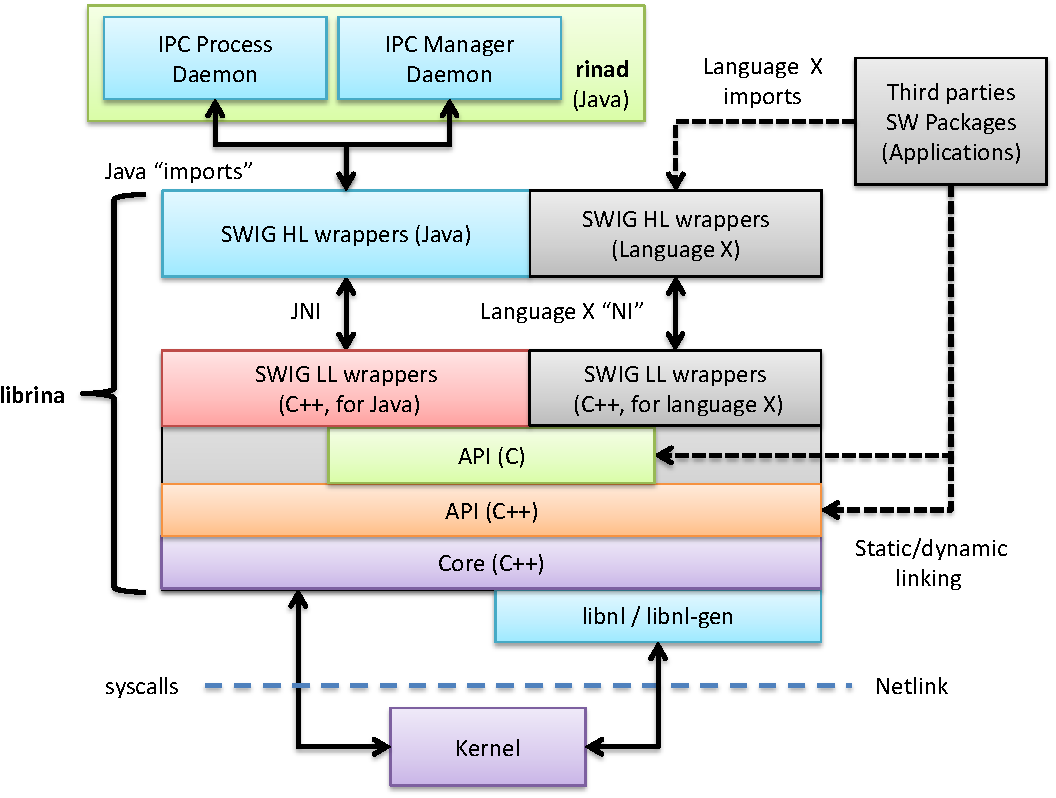
\includegraphics[width=1\textwidth]{figures/userspacearch}
    \caption{Overview of IRATI} 
    \label{fig:userspacearch}
\end{figure}

We see that the section of librina is mostly written in \cpp and then translated to Java functions through SWIG. This is the exact functionality that Android NDK also provides. It provides a environment that allows the developer to code in C or \cpp and translates this code to native libraries which can then be packed in \emph{.apk} files. These are Android specific files which represent programs. However, Android NDK comes with some limitations, as it is built for Android, it is specifically tailored to the Bionic library and does not support glibc. A solution for this is to use a different NDK, such as Crystax NDK\footnote{\url{https://www.crystax.net/en/android/ndk}}. These provide full support for \cpp and would thus perfectly fit for librina. If the kernel could be successfully implemented, the RINA userspace code that is written in \cpp (librina) should be imported in this NDK, adapted to the NDK and then produced as an .apk file. The rinad section (see figure~\ref{fig:userspacearch} above), is written in Java, thus can be copied to Android and be presented as a simple program. Of course, the librina can be imported as a native library then in one bigger program, which would also contain rinad. Given the current state of the IRATI project, this seems the most feasible solution towards implementation on Android.

\subsection{Android specific implementation}

%Specific implementation for the Galaxy S2, select stable kernel (cyanogenmod) and show changes made to add glibc and irati to it. Show if it works on the devices.

Following the previous subsections, this subsection is dedicated to an representation of the entire process. However, as we have noted we have encountered a plethora of difficulties in both kernelspace and userspace. This means that the actual implementation on the physical devices could not be realized and thus the test can not be completed. We do believe that while the original research question states: ``How to implement RINA on Android over WiFi'', we have proven that the WiFi aspect does not matter in this equation and that Android is a very strict platform. 
\npar
Because Android is such a specific platform we can see this research question in a different light. How to expand the IRATI codebase on different Linux-like Operating Systems, possibly with different architectures. In the final subsection of the implementation we address the alternatives that could prove to be helpful. Finally we attempt to show brief implementation processes that could be feasible for these alternatives, concerning RINA.

\subsection{Alternative implementation possibilities}

The final subsection is dedicated to alternatives of implementation. As we have shown during the previous (sub)sections, Android is very restricting. Within the current timeframe it is not possible to acquire a fully working RINA implementation with the IRATI codebase on Android. However we note that while Android is very restricting, other systems might be more viable for implementation of IRATI code. The goal is to stay on the same architecture, ARM. We see that different options become viable alternative paths. These options are:

\begin{itemize}
	\item Ubuntu Touch
	\item Debian next to Android
	\item Debian on Android
	\item Sailfish Operating System 
	\item More recent device
\end{itemize}

\npar

A quick glance over these options show that we are moving closer to less strict environments while still staying on the ARM architecture. While the most promising is most likely Ubuntu Touch, recently the entire development has been halted for the devices (i9100). This makes the Ubuntu Touch option a fairly unpredictable one as no backup or help can be found for the implementation of this. In its current form it is not possible to get the screen working and while Debian and Ubuntu are fairly similar, they are not exactly alike.
\npar
The second option of running Debian next to Android in its own space is a viable one, but has not been done for the device. This means that the same issues arise as the previous option: no help, no developing community, \ldots. While if it would be fairly easy to acquire this might be the best option, but as previously stated: this option falls short when paying respect to the limited timeframe. 
\npar
The third option, Debian on Android, might turn out to be the most interesting one. It has been done and can easily be implemented through Google Play Store. Several options are available such as:

\begin{itemize}
	\item Linux on Android
	\item Debian Kit
	\item Linux Deploy
	\item Complete Linux Installer
	\item \ldots
\end{itemize}

Given the limited timeframe we will attempt to test several of these devices and add our findings later. What we actually require from this: being able to construct our own kernel, if we get a base kernel and modify the IRATI kernel-specific code into this we can move towards the next step. Install this with Debian and attempt to install all the required userspace packages through ``apt-get install'', finally add swig through manual installation. This means that the packages will have to specifically run on ARM, or will have to be general and run on all architectures. Finally we have to note that this means that we are running Debian as a virtual machine on top of Android. This means that even if we can set up VLAN interfaces in the virtual machine, this does not mean that the Android device will use VLAN. More probably: we would have to set up RINA in such a way that we no longer care about VLAN tags, and instantly assume that all traffic is RINA traffic. Only if all these conditions are met will we be able to communicate between the two devices.
\npar
The second to last option that we will address here is the option of looking towards other operating systems that support ARM. Sailfish OS is such an operating system. It is built for ARM devices but ships with a fully fledged glibc library. Furthermore does it still support Android application through an adaptor layer. However, since no such device is physically available for this Master's Thesis we have to consider this option as an alternative, however not a viable alternative at this point of time.
\npar
The final option is simply to update the test devices. They run on kernel version 3.0.101, while newer devices easy run on 3.4.x. The newest devices will soon also start to be built for ARMv8 instead of ARMv7, which could open the doors further for technological improvements. Not only do new devices have more technological options, since they are newer most of these devices will have a bigger, more recent developing community, eager to get their hands on extra implementations. One of these implementations could be to acquire a working RINA on Android.
\npar
We can conclude that even with different alternatives we do not have one clear alternative that offers us the entire solution. While we have acquired plentiful knowledge about the subject and all relevant options, alternatives, \ldots. We have to consider the limited timeframe and scope of this Master's Thesis. The alternatives will be tested but we have to consider the downsides to each of these implementation alternatives.



